\documentclass{article}
\usepackage[margin=0.5in]{geometry}
\usepackage{graphicx}
\usepackage[font={small,it}]{caption}
\usepackage{Sweave}
\begin{document}
\Sconcordance{concordance:latexStatisticsCoursework.tex:latexStatisticsCoursework.Rnw:%
1 7 1 50 0 1 15 6 1 1 4 1 1 1 74 19 1 1 7 9 1 1 19 20 1 5 0 2 1 1 5 1 1 1 6 1 1 %
1 17 15 1}



\title{Statistics Coursework}
\author{Alun Meredith}
\maketitle
\section{Reading data}
Downloaded fish.txt, data about the catch of a hypothetical fishing fleet from:\\"http://www.edshare.soton.ac.uk/view/courses/COMP6235/2015.html" on Thu Oct 22 00:53:41 2015. 
\begin{Schunk}
\begin{Sinput}
> readLines("fish.txt", 5)
\end{Sinput}
\begin{Soutput}
[1] "15.25 2.79 " "13.45 2.69 " "5.58 2.20 "  "7.17 3.21 "  "13.81 2.12 "
\end{Soutput}
\end{Schunk}
From reading the first 5 lines of the file we can see that the data is 2 numeric columns. Each variable is seperated by a single whitespace, there is no header and no apparent NA characters or comment/escape characters. As such we can use the default values of read.table, including the col.names argument to name the variables.
\begin{Schunk}
\begin{Sinput}
> fish <- read.table("fish.txt", col.names = c("times", "size"))
\end{Sinput}
\end{Schunk}
\section{Visualising Data}
\begin{figure}[h]
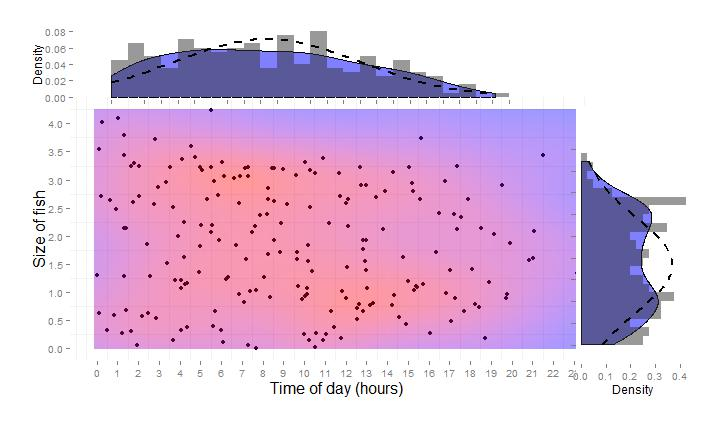
\includegraphics[width=\linewidth]{figure1.jpg}
\caption{\textbf{Bottom Right}: Figure showing scatter graph of size of fish caught vs time of day (hours), coloured background demonstrating a gaussian kernel 2d density \textbf{Right}: Histogram showing distribution of size of fish caught with gaussian kernel density plot overlayed \textbf{Top}: Histogram showing time of day fish caught overlayed by density plot, dashed line shows normal distribution for same mean and standard deviation}
\end{figure}
\begin{Schunk}
\begin{Soutput}
           min             Q1         median             Q3            max           mean 
          0.01           0.94           1.83           2.74           4.23           1.84 
         s.dev       skewness       kurtosis geometric mean 
          1.08           0.09          -1.17           1.37 
\end{Soutput}
\begin{Soutput}
           min             Q1         median             Q3            max           mean 
          0.01           4.88           8.95          13.22          23.16           9.39 
         s.dev       skewness       kurtosis geometric mean 
          5.66           0.25          -0.89           6.79 
\end{Soutput}
\end{Schunk}
By looking at the above summary statistics and the density distributions in the figure, we can see some interesting features of the distributions. The times fish were caught was very broad. A standard deviation of 5.66, along side the mean describes a typical value as anywhere in the range: 3.73. The positive skewness which can be seen in the plot is surprising as you would expect the density at 12:01 to be approximately equal to the density at 11:59. This suggests that an effect such as this data being recorded on a Saturday when no fishing is done on a Sunday is occuring, but requires more domain knowledge to analyse fully. 
The distribution of fish sizes shows a distribution which has some signs of being bi-modal. The standard deviation covers 51.18\% of the data range, which is actually greater than the wide flat times data of 48.9. Both the mean and median sits between the two peaks and there is negligible skewness because the peaks are approximately symmetric and equal in size. 
By assuming an approximation to a normal distribution (t distribution with large degrees of freedom), we can use the t.test function to calcualte confidence intervals. The t.test function makes Bessel's correction automatically.
\begin{Schunk}
\begin{Sinput}
> t.test(times)$conf.int
\end{Sinput}
\begin{Soutput}
[1]  8.599588 10.177112
attr(,"conf.level")
[1] 0.95
\end{Soutput}
\begin{Sinput}
> t.test(size)$conf.int
\end{Sinput}
\begin{Soutput}
[1] 1.692725 1.993375
attr(,"conf.level")
[1] 0.95
\end{Soutput}
\end{Schunk}
We can also map our distributions onto the standard normal curve. The sample distribution mean approximates the mean of the population so we can normalise mean by simply subtracting it. The variance of the sample is given by Bessels correction $s = \sqrt{\frac{\sum{(x-\mu)^2}}{n-1}}$. The variance given by the *var()* function includes Bessel's correction automatically so we just use the *qnorm* function with mean = mean(data) and sd = sqrt(var(data)/n) to compute a confidence interval.
\begin{Schunk}
\begin{Sinput}
> qnorm(c(0.95,0.025), mean = mean(times), sd = sqrt(var(times)/length(times)))
\end{Sinput}
\begin{Soutput}
[1] 10.046274  8.604385
\end{Soutput}
\end{Schunk}
The central figure above shows a scatter of size of fish and time of day. It is hard to identify any dependencies in the data from this but it looks as though it may be slightly weakly correlated. 
\begin{Schunk}
\begin{Sinput}
> cov(times, fish)
\end{Sinput}
\begin{Soutput}
        times       size
[1,] 31.99831 -0.7818909
\end{Soutput}
\begin{Sinput}
> cor(times, fish)
\end{Sinput}
\begin{Soutput}
     times       size
[1,]     1 -0.1282133
\end{Soutput}
\end{Schunk}
You would expect the bigger fish to be easier to catch and therefore some negative correlation to be occuring. The bigger fish will be caught earlier and only the smaller fish left to be caught later. However the correlation is quite small -0.13 and the timescale relatively small we would need mroe domain knowledge to conclude an effect like this. For instance if the fishing is taking place over a larger area (larger population of fish) then the fish caught early in the day will have quite a small effect on the ammount left at the end of the day. 
\section{Intervals}
Splitting the times into 24 intevals corresponding to each hour of the day we can analyse which interval of time has the highest rate of catch (most fish caught that hour) and which has the highest average size of fish. 
\begin{Schunk}
\begin{Sinput}
> #which.max(summary(cut(times, 0:25)))
> intevals <- lapply(0:23, function(x)
+   size[times > x & times <= x+1])
> names(intevals) <- paste("x",paste(0:23, 1:24, sep = "-"), sep="")
> which.max(sapply(intevals, length))
\end{Sinput}
\begin{Soutput}
x12-13 
    13 
\end{Soutput}
\begin{Sinput}
> which.max(sapply(intevals, mean))
\end{Sinput}
\begin{Soutput}
x21-22 
    22 
\end{Soutput}
\end{Schunk}
Looking at this data however we can see that the 21:00-22:00 period has the biggest average fish caught is not what was expected considering the negative correlation calcualted. Looking at each inteval however, this is an outlier as the general trend is that the first third of the day averages around 2 and the last half the day is almsot entirely below 2 (with 2 exceptions). 
\end{document}
